\titledquestion{Pizza Partitioning}

Logan and his good friend Joel want to share a round pizza pie that has been cut into $2n$ equal sector slices along rays from the center at angles $\alpha_i = \frac{i\pi}{n}$ for $i \in \{0,1,...., 2n\}$, where $\alpha_0 = \alpha_{2n}$. Each slice $i$ between angles $\alpha_i$ and $\alpha_{i+1}$ has a known integer tastiness $t_i$ (which might be negative). To be “fair” to her friend, Logan decides to eat slices in the following way:
\begin{itemize}
    \item They will each take turns choosing slices of pizza to eat: Logan starts as the chooser.
    \item If there is only one slice remaining, the chooser eats that slice, and eating stops.
    \item Otherwise the chooser does the following:
    \begin{itemize}
        \item Angle $\alpha_i$ is proper if there is at least one uneaten slice on either side of the line passing
through the center of the pizza at angle $\alpha_i$.
        \item The chooser picks any number $i \in \{1,...,2n\}$ where $\alpha_i$ is proper, and eats all uneaten slices counter-clockwise around the pizza from angle $\alpha_i$ to angle $\alpha_i + \pi$.
    \end{itemize}
\end{itemize}

Logan wants to maximize the total tastiness of the slices she will eat. Describe an $O(n^3)$-time dynamic programming algorithm
to find the maximum total tastiness Logan can guarantee herself via this selection process. 

\textbf{Hints}: \textit{As they eat pizza, the uneaten slices are always cyclically consecutive. That is, each time the chooser eats all uneaten slices within half side, There is no chance that two consecutively parts of pizza are left uneaten. You can choose consecutive cyclic subarrays as the subproblems.}

\begin{figure}[htbp]
    \centering
    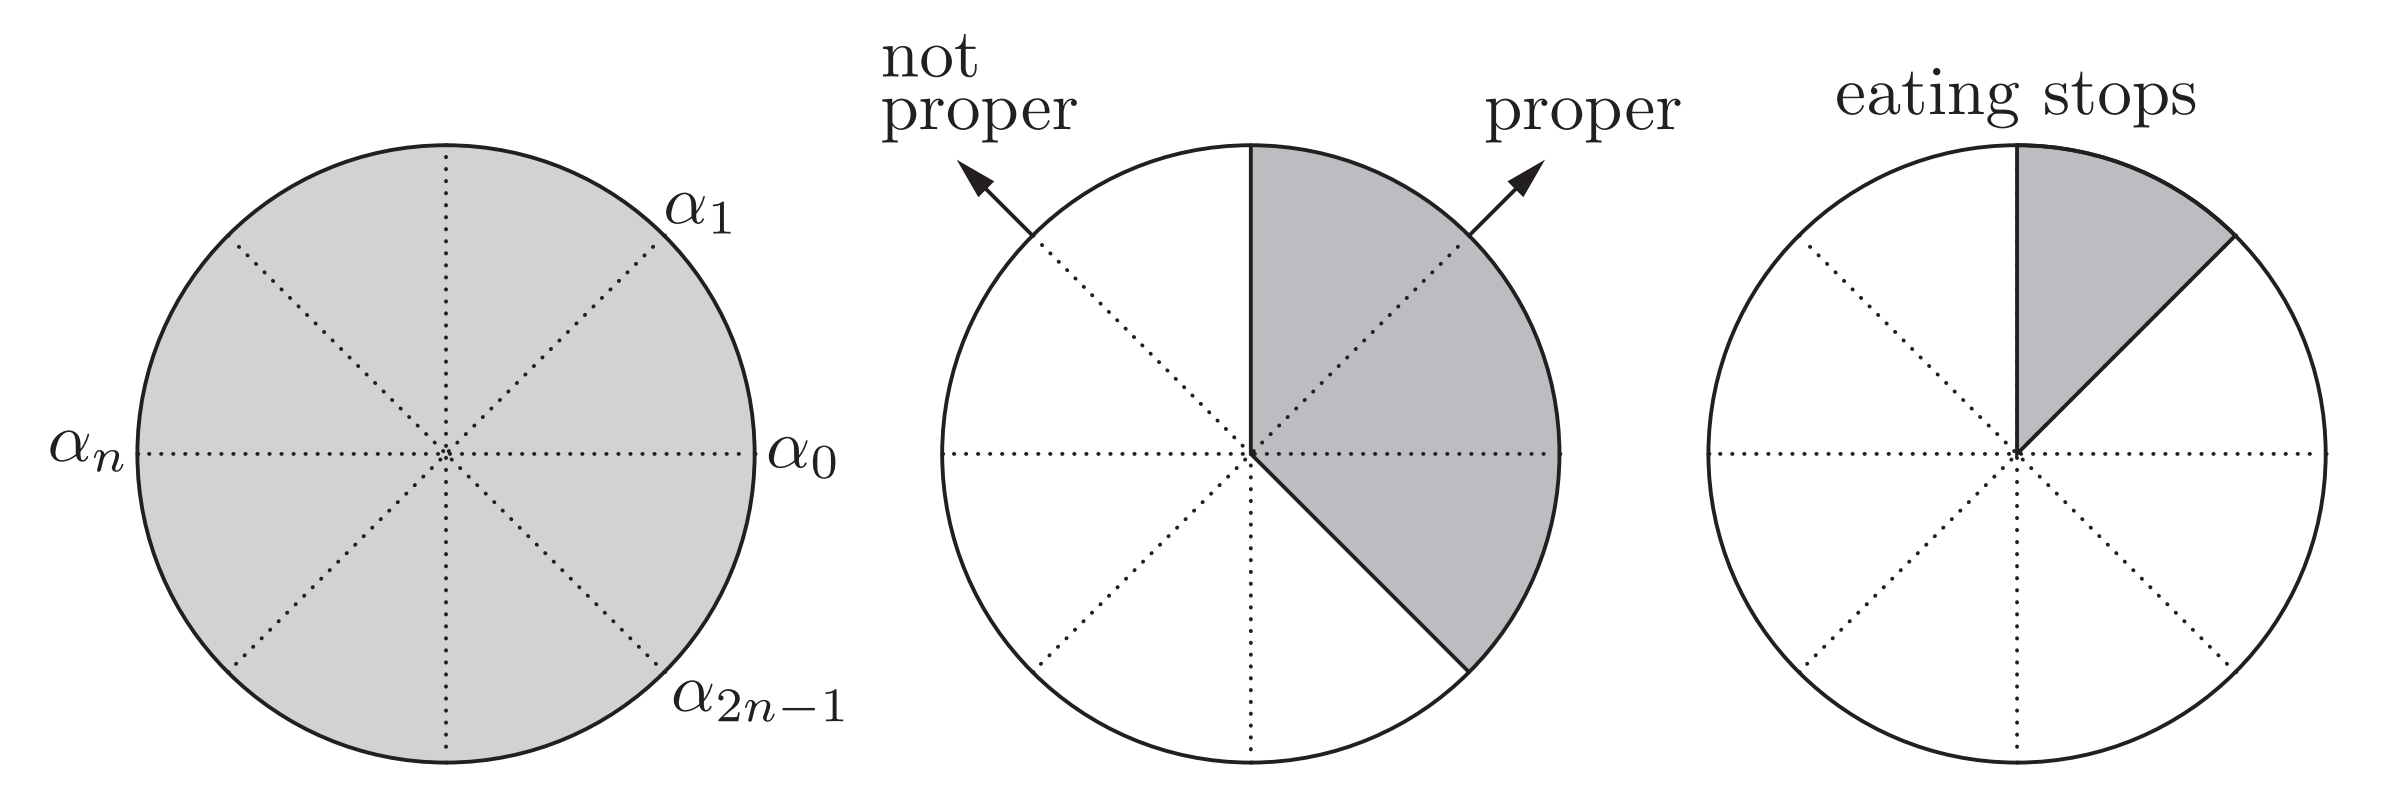
\includegraphics[width=1\linewidth]{p6.png}
\end{figure}

\begin{parts}
    \part[2] As a kickoff, let $v(i, j)$ be the tastiness of the $j$ slices counter-clockwise from angle $\alpha_i$. Write the formula over $v(i, j)$. 

    \begin{solution}
        $v(i, j) = \sum_{k = 0}^{j-1} t_{((i+k) \mod 2n)}$ for $ i \in \{0,1,...,2n-1\}$ and $j \in \{0,1,2,...,n\}$
    \end{solution}

    \part[2] Define your subproblem for this question.

    \begin{solution}
        Define $dp(i, j, p)$ as the maximum total tastiness Logan can guarantee herself with $j$ slices counter-clockwise from angle $\alpha_i$ and $p$ indicating whether it is Logan's turn to choose.(0 for Logan, 1 for Joel)\\
        for $i \in \{0,1,...,2n-1\}$, $j \in \{0,1,2,...,n\}$ and $p \in \{0,1\}$
    \end{solution}

    \bonuspart[4] Give your Bellman equation to solve the subproblems. (Proof of correctness is not required) 

    \begin{solution}
        The Bellman equation is as follows:
        \begin{center}
            $$
            dp(i, j, 0) = \max_{k \in \{1,...,j-1\}} \{\max (v(i, k) + dp(i+k, j-k, 1), v(i + k, j - k) + dp(i,k,1))\} 
            $$\\
            $$
            dp(i, j, 1) = \min_{k \in \{1,...,j-1\}} \{\min (dp(i+k, j-k, 0), dp(i,k,0))\}
            $$
        \end{center}
        for the base case, $dp(i, 1, 0) = v(i, 1)$ and $dp(i, 1, 1) = 0$ for $i \in \{0,1,...,2n-1\}$

    \end{solution}

    \bonuspart[2] What is the answer to this question in terms of the subproblems?

    \begin{solution}
        The answer is $\max_{i \in \{0,1,...,2n-1\}} \{dp(i, n, 1) + v((i+n) \mod 2n, n)\}$
    \end{solution}

    \newpage

    \bonuspart[2] Give an explanation and time complexity analysis of this algorithm.
    \begin{solution}
        \\
        \textbf{Explanation:}
        The total tastiness of all slices is a constant number, so while Logan is maximizing her tastiness, Joel is minimizing his tastiness. We define the subproblem as the maximum total tastiness Logan can guarantee herself with $j$ slices counter-clockwise from angle $\alpha_i$ and $p$ indicating whether it is Logan's turn to choose. From the Hints, we know that the uneaten slices are always cyclically consecutive. So we can choose consecutive cyclic subarrays as the subproblems. We can use the Bellman equation to solve the subproblems. The answer is the maximum total tastiness Logan can guarantee herself.\\
        For each subproblem, chooser can choose any proper angle, for any $k \in \{1,...,j-1\}$, the angle $\alpha_{i+k}$ is proper. And chooser can either eat the slices counter-clockwise from angle $\alpha_i$ to $\alpha_{i+k}$ or from $\alpha_{i+k}$ to $\alpha_{i + j}$. This is because we only require the line passing through the center of the pizza at angle $\alpha_i$ to have at least one uneaten slice on either side. So both choices are valid.
         So we need to consider all possible choices of $k$ and choose the maximum (minimum) tastiness.\\
        \hspace{1cm} \\
        \textbf{Time Complexity:}
        For the initialization of getting $v(i, j)$, it takes $O(n^3)$ time. \\
        For the Bellman equation, we need to consider all possible choices of $k$ for each subproblem, which takes $O(n)$ time. We have $O(n^2)$ subproblems. So the total time complexity is $O(n^3)$.
        Also, we have to compute the final answer, which takes $O(n)$ time.\\
        So the total time complexity is $O(n^3)$.
    \end{solution}

    
\end{parts}